\documentclass[a4paper]{article}

\usepackage[margin=2.5cm]{geometry}
\usepackage{graphicx}

\title{Identification of open loop dynamics of a manually controlled
bicycle-rider system}

\author{Jason K. Moore and Mont Hubbard}

\date{September 30, 2013}

\begin{document}

\maketitle

Traditionally, dynamicists develop models of the bicycle-rider system from
first principles, i.e. Newton's laws and various other atomic fundamental
models of nature. The first principle approach has guided much of engineering
throughout its history but today's experiments are capable of delivering a
staggering amount of both kinematic and kinetic data leading to data driven
modeling approaches.

The Whipple bicycle model is often regarded as a highly predictive model of the
bicycle-rider system and is constructed from first principles, yet very little
experimental data proves that the Whipple model is in fact a robust model for
the open loop dynamics of the bicycle-rider system. Two remedy this, we have
collected a large set of time history data from an instrumented bicycle which
includes the most important kinematic and kinetic variables describing the
bicycle-rider motion from three different riders on the same bicycle for a
variety of maneuvers and speeds. These experiments generated about 1.7 million
time samples from each of about 30 sensors collected at 200 hertz (representing
about 2.4 hours of real time).

The instrumented bicycle was designed so that the riders were not able to move
their legs or torso relative to the rear frame of the bicycle, to ensure that
the assumption of rider rigidity of the Whipple bicycle model was as close to
valid as possible.

We start by simulating the Whipple model given carefully measured physical
parameters and the measured steer torque for each of the 374 runs and show that
the trajectories of the kinematic variables in the simulation are a factor of
magnitude larger than the measurements of those same variables. We conclude
that the Whipple model requires much less steer torque to drive it through the
same trajectory than our real bicycle-rider system.

To rule out the possible invalidations of rigid rider assumptions from allowing
the rider to move his arms while controlling the bicycle we then simulate a
bicycle-rider model with the inertial effects of the rider's arms in the same
fashion as previously described. In general, the model with the arms shows
better agreement to the measured data than does the Whipple model.

Finally, we make use of two structured black box system identification
techniques to identify the coefficients of the Whipple model in both state
space form and mass-spring-damper form. These identification methods result in
various 4th order models that predict the measured data more accurately than
the Whipple model.

\begin{figure}
  \centering
  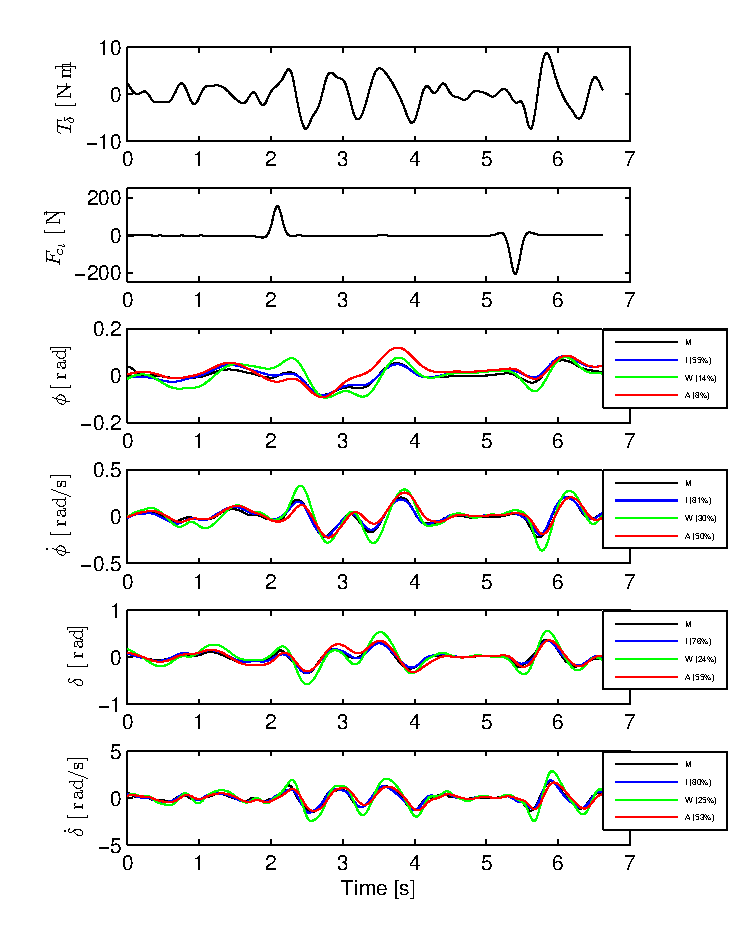
\includegraphics[width=5.0in]{example-fit.pdf}
  \caption{Example results for the identification of a single run (\#596).
    Experimentally measured steer torque and lateral force are shown in the top
    two graphs. The remaining four graphs show the simulation results for the
    Whipple model (W), Whipple model with the arm inertia (A), and the
    identified model for that run (I) plotted with the measured data (M). The
  percentages give the percent of variance explained by each model.}
\end{figure}

In this paper we will show that a fourth order structured state space model is
both adequate for describing the motion of the bicycle under manual control in
a speed range from approximately 1.5 m/s to 9 m/s. The fact that higher order
models may not be necessary for bicycle dynamic description is an important
finding. More robust models of single track vehicles are typically higher than
4th order, with degrees of freedom associated with tire slip, frame
flexibilities, and rider biomechanics. These findings suggest that the more
complex models may be overkill for many modeling purposes.

The data subsequently also reveals that fourth order archetypal first
principles models, such as the Whipple model, are not robust enough to fully
describe the dynamics. The inability to identify realistically valued
parameters and model coefficients points to model deficiencies. The
deficiencies are likely due to un-modeled effects, with the knife-edge, no
side-slip wheel contact assumptions being the most probable candidate.
Un-modeled rider biomechanics such as passive arm stiffness and damping and
head motion may also play a role.

This paper is based on work supported by the National Science Foundation under
Grant No 0928339.

\end{document}
